\chapter{Clustering and Federation}
\label{chap:Clustering}

The initial form of Kestrel as described in Chapter \ref{chap:Kestrel} is
constrained by the use of a single, central manager that imposes both a
bottleneck in task processing and a single point of failure. Two methods for
allowing the use of multiple manager instances are clustering and federation.
There are two primary difference between these methods. The first is the
relationship between the manager instances and any backend storage mechanisms,
and the second is public identity presented by any single manager agent.

\section{Clustering}
A clustering mechanism allows multiple manager instances to share the same
identity, or JID. In addition, each clustered instance will share access to the
same backend data storage service, allowing state to be synchronized between all
instances. The result is effectively a single manager instance that has been
spread across multiple processors. Users and worker agents may interact with
this singular, logical manager with each message handled by a different physical
machine. The loss of a single manager instance within the cluster should not
impact the functionality of the entire cluster, with the exception that any
processing done by that instance at the time of disconnection may be lost and
require re-submission. As such, a clustered system may achieve high availability
by ensuring the continued presence of at least one manager instance in the
cluster at any given moment. An analogous technique would be load balancing for
HTTP servers for the same domain.

\subsection{Challenges with Redis}
For Kestrel, Redis \cite{Redis} was chosen for use as a shared data store between
manager instances for the atomic operations it supports on complex data types such
as dictionaries, sets, and lists. Converting the Kestrel manager to use Redis was
a challenging process:
\begin{itemize}
\item Underlying library support was not written with clustering or use with Redis
in mind.
\item Remapping the current SQL database schema to the data structures provided by Redis.
\item New algorithms for matching workers and jobs based on job requirements and worker
capabilities were needed to match the new data storage patterns. The previous algorithm
relied on SQL's \texttt{LIKE} operation which is not available with Redis.
\item The data which had to be stored in Redis was not data that could be stored easily,
such as callback functions or other closures.
\item The load balancing offered by the XMPP server routed incoming messages to a random
manager instance. Thus the instance that sends an \texttt{<iq />} stanza was not
necessarily the same instance that would receive the reply.
\end{itemize}

\subsection{Library Support}
The first step in implementing clustering support was enabling the underlying
SleekXMPP library used by Kestrel to work in such an arrangement. The SleekXMPP
plugins that provided support for rosters, service discovery, and ad-hoc commands
were originally created with the assumption of running in a single process,
and used simple in-memory data structures for session state and storage as a
result. Thus adding support for external data storage, and the adaptors for
working specifically with Redis was needed. These adaptors have been turned into
a sister library for SleekXMPP, named SleekRedis \cite{SleekRedis}.

Most of the work done was to build in hooks for using generic external
data storage mechanisms, and make explicit interfaces for how new storage
mechanisms could be added. In the case of ad-hoc commands, the session data was
originally stored in a Python dictionary. Since custom classes may implement the
\texttt{\_\_getitem\_\_}, \texttt{\_\_setitem\_\_}, and \texttt{\_\_delitem\_\_}
methods to provide support for the dictionary syntax, adding the external
storage support was easier.

\subsection{Mapping SQL databases to Redis}
The second challenge was representing all of the data from the older SQL
database to Redis key-value pairs. Whereas in a SQL table one may have a
field to mark an entry as \texttt{AVAILABLE} or \texttt{BUSY}, the pattern in
Redis is to create sets for each option. Thus, for workers there are the sets
\texttt{workers:available}, \texttt{workers:online}, and \texttt{workers:busy},
each of which contains the JIDs of the relevant worker agents. However, this
caused the proliferation of keys and sets to segregate workers and jobs in
their various states of execution. To ensure that all related keys were updated
appropriately for changes in a job or worker's state, the use of Redis'
pipelines were required. A pipeline is similar to a transaction in a typical
SQL database with ACID support. While each individual Redis command is atomic,
a pipeline enqueue multiple commands and ensures that the entire sequence is
executed atomically.

\begin{lstlisting}[
    language=Python,
    label=fig:Job-Matching,
    caption={The code for determining the set of available workers to available
    tasks for a given job.},
    float=hh
]
def job_matches(self, job):
    requirements = self.redis.smembers('job:%s:requirements' % job)
    p = self.redis.pipeline()
    matches = {}
    workers = self.redis.smembers('job:%s:workers' % job)
    for worker in workers:
        if self.redis.sismember('workers:available', worker):
            task = self.redis.srandmember('job:%s:tasks:queued' % job)
            if task is not None:
                p.smove('job:%s:tasks:queued' % job,
                        'job:%s:tasks:pending' % job,
                        task)
                p.set('job:%s:task:%s:is_pending' % (job, task), 'True')
                p.expire('job:%s:task:%s:is_pending' % (job, task), 15)
                p.sadd('worker:%s:tasks' % worker,
                       '%s,%s' % (job, task))
                p.set('job:%s:task:%s' % (job, task), worker)
                log.debug('MATCH: Matched worker %s to ' % worker + \
                          'task %s,%s' % (job, task))
                matches[task] = worker
    p.execute()
    return matches
\end{lstlisting}

\subsection{Matching Jobs with Workers}
The process for matching a worker with a job, and vice versa, was performed using
a \texttt{LIKE} query in the SQLite database, but there is no equivalent command
in Redis. By rephrasing the problem, a Redis compatible method was found. Instead
of performing a search whenever a match is needed, all possible matches are computed
whenever a worker is added to the pool, or a job is submitted. The sets of matching
job IDs are stored for each worker, and likewise for each job. When a match is
requested, a random member of the applicable set is selected and checked for
availability.

Listing \ref{fig:Job-Matching} shows the process of matching workers to tasks for
a given job. First, the set of known workers suitable for the job is retrieved. For
each available worker, a task is randomly chosen and assigned to the worker, marking
the task as pending. Redis provides support for expiring key values after a given delay;
the feature is used here to indicate the allowable time to wait for a task assignment
to be acknowledged by the worker. A periodic cleanup function exams all tasks marked as 
pending and if the associated \texttt{is\_pending} key is not found, then the assignment
has timed out and must be reset.

\subsection{Serialization}
The largest hurdle was dealing with data that could not be serialized. In particular,
Python's \texttt{pickle} facility for serializing code objects will not serialize
object methods, and it can not unserialize functions that were created on-the-fly.
The trouble was that those types of entities were used heavily for ad-hoc commands,
which stored function pointers to callback functions. The first attempt at resolving
this was to remove the use of on-the-fly generated functions and use only defined
object methods. After that change, an attempt was made to add support for serializing
methods. Existing code to perform this operation was found from the Twisted Python
project \cite{Twisted}. However, the underlying SleekXMPP library still required the use of a
generated function, which prevented unserializing the stored methods.

An initial goal of adding Redis support to the ad-hoc commands plugin was to make the
support transparent to an end user. However, as a compromise the current approach
is to initialize the plugin with all of the potential callback functions. The plugin
then hashes the names of the functions and stores the mapping in memory. It is the hash
of the function's name that is stored if a function is detected in the session data to be stored
in Redis. The current limitation to this approach is that using different
methods with the same name will not work as expected. Situations like this would occur
if one callback was the method \texttt{do\_foo} of object \texttt{a}, and a second
callback of method \texttt{do\_foo} of object \texttt{b} were registered.

Other serialization issues included restoring stanza and JID objects. Upon unserializing
the objects, errors would occur because the necessary classes were not loaded. To resolve
this, instead of serializing the objects directly, the underlying data was extracted and
saved. Each key in the session data dictionary that required this treatment was saved in
a list in a special \texttt{\_\_XML\_\_}, \texttt{\_\_JID\_\_}, or \texttt{\_\_FUNC\_\_} key.

\subsection{XMPP Server Load Balancing}
XMPP server implementations, in particular ejabberd, can provide support for load
balancing external server components, such as the Kestrel manager. The method for
balancing was to route an XMPP stanza to a manager instance based on the stanza's
sender. Thus a single instance would always receive requests from a given client agent.
The problem arose when a different instance sent a message to a client; it was the
other instance that would receive the reply. Thus every manager instance had to be
prepared to receive responses to queries that it did not send. The main culprit
for these situations was the use of ad-hoc commands. With the changes described above
for serializing code objects, it was possible for each manager to retrieve the
original query data whenever a response was received.

\section{Federation}
Federation is a mechanism for allowing separate manager instances to share
information while retaining separate identities. An implication of a clustered
model is that the clustered instances all belong to the same organization, in
contrast to the federated model which allows manager instances from various
organizations to interact. Also, unlike clustering, federation does not
necessitate the persistence of data in the event that an instance goes
offline. Examples of federated systems would be SMTP and XMPP servers.

Implementing federation for Kestrel was more straightforward than clustering
since syncing state using Redis was not needed. The method of federation chosen
for Kestrel was to allow a manager to share tasks with another manager by
masquerading as a worker. The lifecycle for federation between manager $M_1$ and
$M_2$ is as follows:
\begin{enumerate}
\item $M_1$ is instructed to federate with $M_2$.
\item For each unique set of features supported by the workers for $M_1$,
$M_1$ registers as a virtual worker to $M_2$, with the addition of the feature
\texttt{kestrel:federation}.
\item $M_2$ begins dispatching tasks to the virtual ``workers.'' The
\texttt{kestrel:federation} feature may be used by $M_2$ to only dispatch to
virtual workers when no local workers are available.
\item $M_1$ forwards received tasks to its own available workers (or potentially other managers).
\item If all workers providing a given set of features are all busy, $M_1$ may
send $M_2$ a busy presence notice to prevent receiving new tasks requiring those
features.
\item $M_1$ sends a task complete notice to $M_2$ when the task is completed,
following the standard worker protocol.
\end{enumerate}

Note that if the manager $M_2$ goes offline it is not required that $M_1$ take
responsibility for any jobs tracked by $M_2$. Using both clustering and federation
can ensure continued task tracking after the loss of a given instance. Also note that
step 4, where $M_1$ forwards a task to a worker, can create an infinite loop if both
$M_1$ and $M_2$ are mutually registered as workers. Such an arrangement may be partially
avoided by having each manager refuse to forward a task back to the manager from which
the task was received. Situations where a larger loop is created, as shown in figure
\ref{fig:Federated-Loop}, may require other special handling. One possibility would
be to simply mark a task as not to be forwarded after a certain number of hops.

The result of federation can effectively turn manager instances into routers,
or congregators for workers. Such an architecture as shown in figure
\ref{fig:Federated-Tree} could use a manager for each unique set of worker
features such that each manager is responsible for a homogeneous set of workers,
turning it into a simple queue of tasks without any need for matching. A higher,
federated manager instance may then perform matching and track state of a smaller
number of workers, albeit virtual ones. The arrangement in \ref{fig:Federated-Loop}
allows all managers to have access to every worker in the global pool by establishing
a loop. 

\begin{figure}
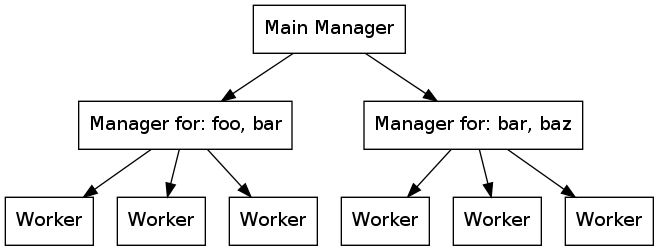
\includegraphics[width=\columnwidth]{figures/federated_tree}
\label{fig:Federated-Tree}
\caption{Layering federated manager instances intro a tree architecture.}
\end{figure}

\begin{figure}
\begin{center}
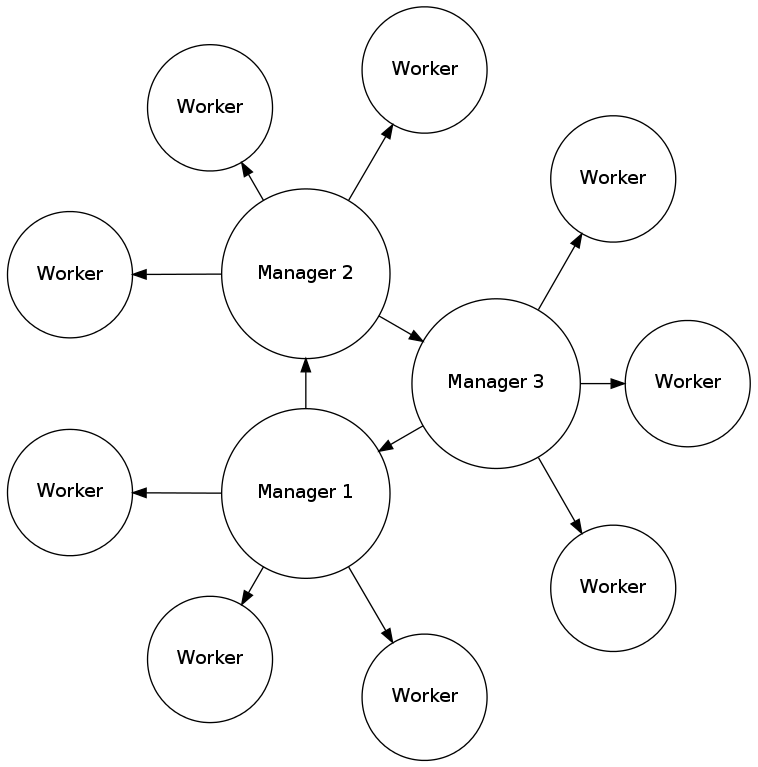
\includegraphics[width=.5\columnwidth]{figures/federated_loop}
\end{center}
\label{fig:Federated-Loop}
\caption{Creating cycles in the federation links between managers means that all managers in the
cycle have access to all of the workers tracked by the managers in the loop. It becomes possible
for a task to then be forwarded endlessly around the loop; therefore, a task should be marked with
the number of hops it has made and once it has reached a configured limit, not be forwarded any
further.}
\end{figure}

